\documentclass{standalone}
\usepackage{tikz}
\usepackage{pgfplots}
\usetikzlibrary{arrows}
\usetikzlibrary{matrix}

%\usetikzlibrary{...}
\begin{document}
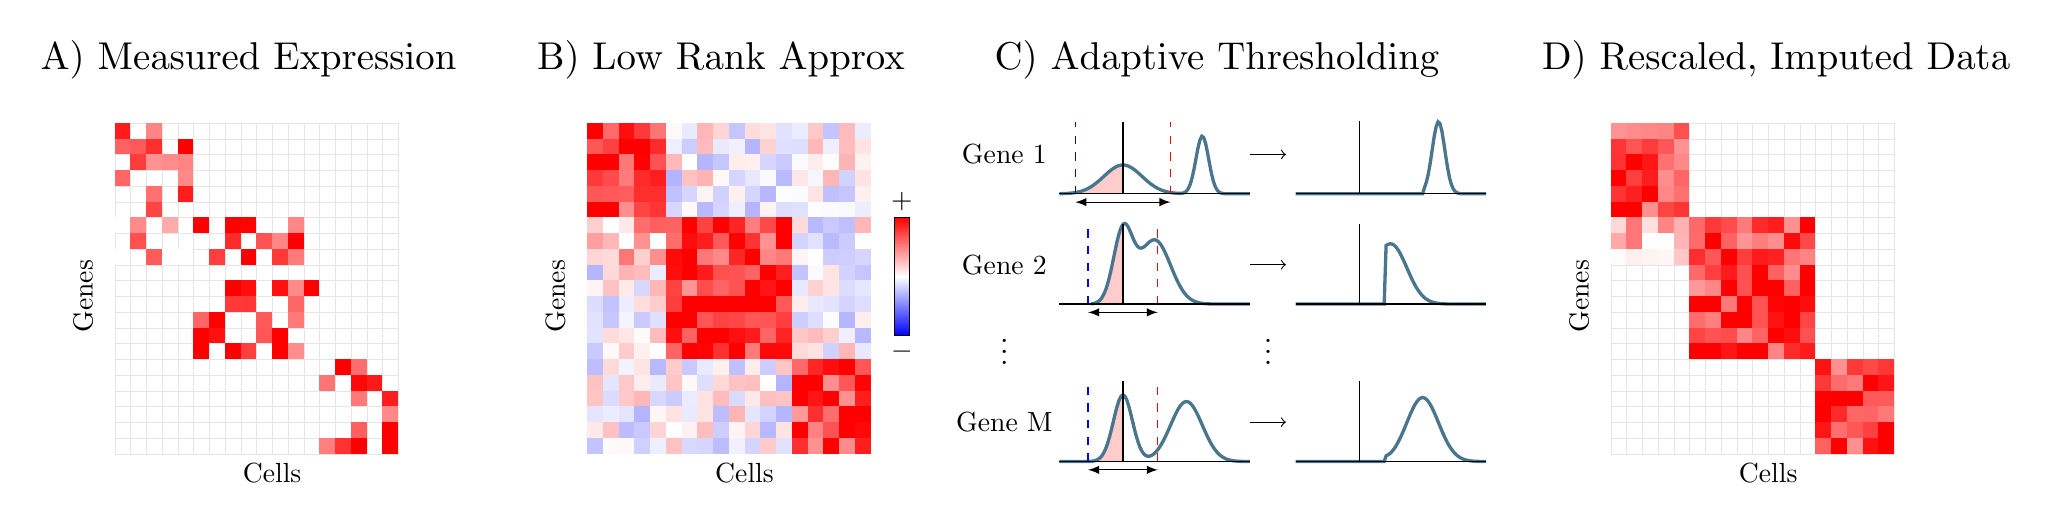
\begin{tikzpicture}[thin, every node/.style={transform shape}]


\begin{scope}[shift={(0,0)}]
\foreach \y in {0.0,0.2,...,4} {
\foreach \x in {0.0,0.2,...,3.4} {
          \path[fill=none,draw=black!10, line width=0.01pt] (\x,\y) rectangle ++(0.2,0.2);
}
}

	\node[scale=1.4] at (1.7,5) {A) Measured Expression};

\pgfmathsetseed{3}

   \def \p {0.6}
  \foreach \y in {3.0,3.2,...,4} {
      \foreach \x in {0.0,0.2,...,0.8} {
       \pgfmathparse{rnd < \p ? 1 : 0}
       \ifnum \pgfmathresult=0
          \pgfmathparse{0.9*rnd-0.3}
          \definecolor{MyColor}{rgb}{1,\pgfmathresult,\pgfmathresult}
          \path[fill=MyColor] (\x,\y) rectangle ++(0.2,0.2);
	\fi
      }
  }

  \foreach \y in {2.4,2.6,...,3.0} {
      \foreach \x in {0.0,0.2,...,0.8} {
       \pgfmathparse{rnd < \p ? 1 : 0}
       \ifnum \pgfmathresult=0
          \pgfmathparse{0.9*rnd+0.3}
          \definecolor{MyColor}{rgb}{1,\pgfmathresult,\pgfmathresult}
          \path[fill=MyColor] (\x,\y) rectangle ++(0.2,0.2);
	\fi
      }
      \foreach \x in {1.0,1.2,...,2.4} {
       \pgfmathparse{rnd < \p ? 1 : 0}
       \ifnum \pgfmathresult=0
          \pgfmathparse{0.9*rnd-0.3}
          \definecolor{MyColor}{rgb}{1,\pgfmathresult,\pgfmathresult}
          \path[fill=MyColor] (\x,\y) rectangle ++(0.2,0.2);
	\fi
      }
  }

  \foreach \y in {1.2,1.4,...,2.2} {
      \foreach \x in {1.0,1.2,...,2.4} {
       \pgfmathparse{rnd < \p ? 1 : 0}
       \ifnum \pgfmathresult=0
          \pgfmathparse{0.9*rnd-0.3}
          \definecolor{MyColor}{rgb}{1,\pgfmathresult,\pgfmathresult}
          \path[fill=MyColor] (\x,\y) rectangle ++(0.2,0.2);
	\fi
      }
  }

  \foreach \y in {0.0,0.2,...,1.0} {
      \foreach \x in {2.6,2.8,...,3.4} {
	\pgfmathparse{rnd < \p ? 1 : 0}
       \ifnum \pgfmathresult=0
          \pgfmathparse{0.9*rnd-0.3}
          \definecolor{MyColor}{rgb}{1,\pgfmathresult,\pgfmathresult}
          \path[fill=MyColor] (\x,\y) rectangle ++(0.2,0.2);
	\fi
      }
  }


\node[rotate=90] at (-0.4,2) {Genes};
\node at (2,-0.25) {Cells};
\end{scope}
\begin{scope}[shift={(6,0)}]

	\node[scale=1.4] at (1.7,5) {B) Low Rank Approx};

   \def \p {0.5}
\pgfmathsetseed{3}
  \foreach \y in {3.0,3.2,...,4} {
      \foreach \x in {0.0,0.2,...,0.8} {
          \pgfmathparse{0.9*rnd-0.3}
          \definecolor{MyColor}{rgb}{1,\pgfmathresult,\pgfmathresult}
          \path[fill=MyColor] (\x,\y) rectangle ++(0.2,0.2);
      }
      \foreach \x in {1.0,1.2,...,3.4} {
          \pgfmathparse{rnd < 0.5 ? 1 : 0}
	       \ifnum \pgfmathresult=0
               \pgfmathparse{0.3*rnd+0.7}\definecolor{MyColor}{rgb}{\pgfmathresult,\pgfmathresult,1};
	       \else
                \pgfmathparse{0.3*rnd+0.7}\definecolor{MyColor}{rgb}{1,\pgfmathresult,\pgfmathresult};
		\fi

          \path[fill=MyColor] (\x,\y) rectangle ++(0.2,0.2);
      }

  }

  \foreach \y in {2.4,2.6,...,3.0} {
      \foreach \x in {0.0,0.2,...,0.8} {
          \pgfmathparse{0.9*rnd+0.3}
          \definecolor{MyColor}{rgb}{1,\pgfmathresult,\pgfmathresult}
          \path[fill=MyColor] (\x,\y) rectangle ++(0.2,0.2);
      }
      \foreach \x in {1.0,1.2,...,2.4} {
          \pgfmathparse{0.9*rnd-0.3}
          \definecolor{MyColor}{rgb}{1,\pgfmathresult,\pgfmathresult}
          \path[fill=MyColor] (\x,\y) rectangle ++(0.2,0.2);
      }
      \foreach \x in {2.6,2.8,...,3.4} {
          \pgfmathparse{rnd < 0.5 ? 1 : 0}
	       \ifnum \pgfmathresult=0
               \pgfmathparse{0.3*rnd+0.7}\definecolor{MyColor}{rgb}{\pgfmathresult,\pgfmathresult,1};
	       \else
                \pgfmathparse{0.3*rnd+0.7}\definecolor{MyColor}{rgb}{1,\pgfmathresult,\pgfmathresult};
		\fi

          \path[fill=MyColor] (\x,\y) rectangle ++(0.2,0.2);
      }
  }

  \foreach \y in {1.2,1.4,...,2.2} {
      \foreach \x in {0.0,0.2,...,0.8} {
          \pgfmathparse{rnd < 0.5 ? 1 : 0}
	       \ifnum \pgfmathresult=0
               \pgfmathparse{0.3*rnd+0.7}\definecolor{MyColor}{rgb}{\pgfmathresult,\pgfmathresult,1};
	       \else
                \pgfmathparse{0.3*rnd+0.7}\definecolor{MyColor}{rgb}{1,\pgfmathresult,\pgfmathresult};
		\fi

          \path[fill=MyColor] (\x,\y) rectangle ++(0.2,0.2);
      }
      \foreach \x in {1.0,1.2,...,2.4} {
          \pgfmathparse{0.9*rnd-0.3}
          \definecolor{MyColor}{rgb}{1,\pgfmathresult,\pgfmathresult}
          \path[fill=MyColor] (\x,\y) rectangle ++(0.2,0.2);
      }
      \foreach \x in {2.6,2.8,...,3.4} {
          \pgfmathparse{rnd < 0.5 ? 1 : 0}
	       \ifnum \pgfmathresult=0
               \pgfmathparse{0.3*rnd+0.7}\definecolor{MyColor}{rgb}{\pgfmathresult,\pgfmathresult,1};
	       \else
                \pgfmathparse{0.3*rnd+0.7}\definecolor{MyColor}{rgb}{1,\pgfmathresult,\pgfmathresult};
		\fi

          \path[fill=MyColor] (\x,\y) rectangle ++(0.2,0.2);
      }
  }

  \foreach \y in {0.0,0.2,...,1.0} {
      \foreach \x in {0.0,0.2,...,2.6} {
          \pgfmathparse{rnd < 0.5 ? 1 : 0}
	       \ifnum \pgfmathresult=0
               \pgfmathparse{0.3*rnd+0.7}\definecolor{MyColor}{rgb}{\pgfmathresult,\pgfmathresult,1};
	       \else
                \pgfmathparse{0.3*rnd+0.7}\definecolor{MyColor}{rgb}{1,\pgfmathresult,\pgfmathresult};
		\fi

          \path[fill=MyColor] (\x,\y) rectangle ++(0.2,0.2);
      }
      \foreach \x in {2.6,2.8,...,3.4} {
          \pgfmathparse{0.9*rnd-0.3}
          \definecolor{MyColor}{rgb}{1,\pgfmathresult,\pgfmathresult}
          \path[fill=MyColor] (\x,\y) rectangle ++(0.2,0.2);
      }
  }

  %\draw[step=.3,help lines] (0,0) grid (3,4);

\node[rotate=90] at (-0.4,2) {Genes};
\node at (2,-0.25) {Cells};
    %\node [rectangle, bottom color=white, top color=red, minimum width=0.5, minimum height=5] (box) at (4,2){};
    \draw[top color=red,bottom color=blue,middle color=white]
  (3.9,1.5) rectangle (4.1,3);
  \node at (4.0,3.2) {$+$};
  \node at (4.0,1.3) {$-$};


\end{scope}


\def \densstartx {12}
\def \genex {-.7}
\def \geney {0.5}

%%% Density 1
\node[scale=1.4] at (14,5) {C) Adaptive Thresholding};
\begin{scope}[shift={(\densstartx,3.3)}]
\pgfmathdeclarefunction{gauss}{2}{%
  \pgfmathparse{1/(#2*sqrt(2*pi))*exp(-((x-#1)^2)/(2*#2^2))}%
}

\pgfmathdeclarefunction{gauss2}{4}{%
  \pgfmathparse{1.5/(#2*sqrt(2*pi))*exp(-((x-#1)^2)/(2*#2^2))+1/(#4*sqrt(2*pi))*exp(-((x-#3)^2)/(2*#4^2)) }%
}
\begin{axis}[
  no markers, domain=-2:4, samples=100,
  axis y line*=middle,  axis x line*=bottom,
  every axis y label/.style={at=(current axis.above origin),anchor=south},
  every axis x label/.style={at=(current axis.right of origin),anchor=west},
  height=2.5cm, width=4cm,
  xtick=\empty, ytick=\empty,
  enlargelimits=false, clip=false, axis on top,
  grid = major
  ]
  \addplot [fill=red!20, draw=none, domain=-2:0] {gauss2(0,0.6,2.5,0.2)} \closedcycle;
\addplot [very thick,cyan!50!black] {gauss2(0,0.6,2.5,0.2)};

  \addplot[mark=none, black,dashed,color=blue] coordinates {(-1.5,0) (-1.5,2.5)};
  \addplot[mark=none, black,dashed,color=red] coordinates {(1.5,0) (1.5,2.5)};
  \draw [yshift=-3, latex-latex](axis cs:-1.5,0) --  (axis cs:1.5,0);
\end{axis}
\node at (\genex,\geney) {Gene 1};
	\node at (2.3,0.5) (A) {};
	\node at (3,0.5) (B){};
	\draw[->] (A) edge (B);
\end{scope}

\begin{scope}[shift={(\densstartx+3,3.3)}]
\pgfmathdeclarefunction{gauss}{2}{%
  \pgfmathparse{1/(#2*sqrt(2*pi))*exp(-((x-#1)^2)/(2*#2^2))}%
}

      %\pgfmathparse{\i*#4-\j > -1 ? 1 : 0}
\pgfmathdeclarefunction{gauss2}{4}{%
  \pgfmathparse{x > 2 ?1/(#2*sqrt(2*pi))*exp(-((x-#1)^2)/(2*#2^2))+1/(#4*sqrt(2*pi))*exp(-((x-#3)^2)/(2*#4^2)): 0 }%
}
\begin{axis}[
  no markers, 
	ymin=0,ymax=2,
	domain=-2:4, samples=100,
  axis y line*=middle,  axis x line*=bottom,
  every axis y label/.style={at=(current axis.above origin),anchor=south},
  every axis x label/.style={at=(current axis.right of origin),anchor=west},
  height=2.5cm, width=4cm,
  xtick=\empty, ytick=\empty,
  enlargelimits=false, clip=false, axis on top,
  grid = major
  ]
  \addplot [fill=red!20, draw=none, domain=-2:0] {gauss2(0,0.6,2.5,0.2)} \closedcycle;
\addplot [very thick,cyan!50!black] {gauss2(0,0.6,2.5,0.2)};

\end{axis}
\end{scope}

%%% Density 2
\begin{scope}[shift={(\densstartx,1.9)}]
\pgfmathdeclarefunction{gauss}{2}{%
  \pgfmathparse{1/(#2*sqrt(2*pi))*exp(-((x-#1)^2)/(2*#2^2))}%
}

\pgfmathdeclarefunction{gauss2}{4}{%
  \pgfmathparse{1/(#2*sqrt(2*pi))*exp(-((x-#1)^2)/(2*#2^2))+1.5/(#4*sqrt(2*pi))*exp(-((x-#3)^2)/(2*#4^2)) }%
}
\begin{axis}[
  no markers, domain=-1:4, samples=100,
	ymin=0,ymax=1.5,
  axis y line*=middle,  axis x line*=bottom,
  every axis y label/.style={at=(current axis.above origin),anchor=south},
  every axis x label/.style={at=(current axis.right of origin),anchor=west},
  height=2.6cm, width=4cm,
  xtick=\empty, ytick=\empty,
  enlargelimits=false, clip=false, axis on top,
  grid = major
  ]
  \addplot [fill=red!20, draw=none, domain=-2:0] {gauss2(0,0.3,1,0.5)} \closedcycle;
\addplot [very thick,cyan!50!black] {gauss2(0,0.3,1,0.5)};
  \addplot[mark=none, black,dashed,color=blue] coordinates {(-1.1,0) (-1.1,1.5)};
  \addplot[mark=none, black,dashed,color=red] coordinates {(1.1,0) (1.1,1.5)};
  \draw [yshift=-3, latex-latex](axis cs:-1.1,0) --  (axis cs:1.1,0);

\end{axis}
\node at (\genex,\geney) {Gene 2};
	\node at (2.3,0.5) (A) {};
	\node at (3,0.5) (B){};
	\draw[->] (A) edge (B);
\end{scope}

\begin{scope}[shift={(\densstartx+3,1.9)}]
\pgfmathdeclarefunction{gauss}{2}{%
  \pgfmathparse{1/(#2*sqrt(2*pi))*exp(-((x-#1)^2)/(2*#2^2))}%
}

      %\pgfmathparse{\i*#4-\j > -1 ? 1 : 0}
\pgfmathdeclarefunction{gauss2}{4}{%
  \pgfmathparse{x > 0.8 ?1/(#2*sqrt(2*pi))*exp(-((x-#1)^2)/(2*#2^2))+1.5/(#4*sqrt(2*pi))*exp(-((x-#3)^2)/(2*#4^2)): 0 }%
}
\begin{axis}[
  no markers, domain=-2:4, samples=100,
	ymin=0,ymax=1.6,
  axis y line*=middle,  axis x line*=bottom,
  every axis y label/.style={at=(current axis.above origin),anchor=south},
  every axis x label/.style={at=(current axis.right of origin),anchor=west},
  height=2.6cm, width=4cm,
  xtick=\empty, ytick=\empty,
  enlargelimits=false, clip=false, axis on top,
  grid = major
  ]
  \addplot [fill=red!20, draw=none, domain=-2:0] {gauss2(0,0.3,2,0.5)} \closedcycle;
\addplot [very thick,cyan!50!black] {gauss2(0,0.3,1,0.5)};

\end{axis}
\end{scope}



%%% Density 3
\begin{scope}[shift={(\densstartx,-0.1)}]
\pgfmathdeclarefunction{gauss}{2}{%
  \pgfmathparse{1/(#2*sqrt(2*pi))*exp(-((x-#1)^2)/(2*#2^2))}%
}

\pgfmathdeclarefunction{gauss2}{4}{%
  \pgfmathparse{1/(#2*sqrt(2*pi))*exp(-((x-#1)^2)/(2*#2^2))+1.5/(#4*sqrt(2*pi))*exp(-((x-#3)^2)/(2*#4^2)) }%
}
\begin{axis}[
  no markers, domain=-2:4, samples=100,
	ymin=0,ymax=1.6,
  axis y line*=middle,  axis x line*=bottom,
  every axis y label/.style={at=(current axis.above origin),anchor=south},
  every axis x label/.style={at=(current axis.right of origin),anchor=west},
  height=2.6cm, width=4cm,
  xtick=\empty, ytick=\empty,
  enlargelimits=false, clip=false, axis on top,
  grid = major
  ]
  \addplot [fill=red!20, draw=none, domain=-2:0] {gauss2(0,0.3,2,0.5)} \closedcycle;
\addplot [very thick,cyan!50!black] {gauss2(0,0.3,2,0.5)};
  \addplot[mark=none, black,dashed,color=blue] coordinates {(-1.1,0) (-1.1,1.5)};
  \addplot[mark=none, black,dashed,color=red] coordinates {(1.1,0) (1.1,1.5)};
  \draw [yshift=-3, latex-latex](axis cs:-1.1,0) --  (axis cs:1.1,0);
  %\draw [yshift=-3, latex-latex](axis cs:-1.1,0) -- node [fill=white,scale=0.5] {$0$} (axis cs:1.1,0);




\end{axis}

\node at (\genex,1.5) {\large \vdots};
\node at (\genex,\geney) {Gene M};
	\node at (2.3,0.5) (A) {};
	\node at (3,0.5) (B){};
	\draw[->] (A) edge (B);
	\node at (2.65,1.5) {\large \vdots};
\end{scope}

\begin{scope}[shift={(\densstartx+3,-0.1)}]
\pgfmathdeclarefunction{gauss}{2}{%
  \pgfmathparse{1/(#2*sqrt(2*pi))*exp(-((x-#1)^2)/(2*#2^2))}%
}

      %\pgfmathparse{\i*#4-\j > -1 ? 1 : 0}
\pgfmathdeclarefunction{gauss2}{4}{%
  \pgfmathparse{ x > 0.8 ? 1/(#2*sqrt(2*pi))*exp(-((x-#1)^2)/(2*#2^2))+1.5/(#4*sqrt(2*pi))*exp(-((x-#3)^2)/(2*#4^2)) : 0 }%
}
\begin{axis}[
  no markers, domain=-2:4, samples=100,
  axis y line*=middle,  axis x line*=bottom,
	ymin=0,ymax=1.5,
  every axis y label/.style={at=(current axis.above origin),anchor=south},
  every axis x label/.style={at=(current axis.right of origin),anchor=west},
  height=2.6cm, width=4cm,
  xtick=\empty, ytick=\empty,
  enlargelimits=false, clip=false, axis on top,
  grid = major
  ]
  \addplot [fill=red!20, draw=none, domain=-2:0] {gauss2(0,0.3,2,0.5)} \closedcycle;
\addplot [very thick,cyan!50!black] {gauss2(0,0.3,2,0.5)};

\end{axis}
\end{scope}
\begin{scope}[shift={(19,0)}]

	\node[scale=1.4] at (2.1,5) {D) Rescaled, Imputed Data};
\foreach \y in {0.0,0.2,...,4} {
\foreach \x in {0.0,0.2,...,3.4} {
          \path[fill=none,draw=black!10, line width=0.01pt] (\x,\y) rectangle ++(0.2,0.2);
}
}

\pgfmathsetseed{3}
  \foreach \y in {3.0,3.2,...,4} {
      \foreach \x in {0.0,0.2,...,0.8} {
          \pgfmathparse{0.9*rnd-0.3}
          \definecolor{MyColor}{rgb}{1,\pgfmathresult,\pgfmathresult}
          \path[fill=MyColor] (\x,\y) rectangle ++(0.2,0.2);
      }
  }

  \foreach \y in {2.4,2.6,...,3.0} {
      \foreach \x in {0.0,0.2,...,0.8} {
          \pgfmathparse{0.9*rnd+0.3}
          \definecolor{MyColor}{rgb}{1,\pgfmathresult,\pgfmathresult}
          \path[fill=MyColor] (\x,\y) rectangle ++(0.2,0.2);
      }
      \foreach \x in {1.0,1.2,...,2.4} {
          \pgfmathparse{0.9*rnd-0.3}
          \definecolor{MyColor}{rgb}{1,\pgfmathresult,\pgfmathresult}
          \path[fill=MyColor] (\x,\y) rectangle ++(0.2,0.2);
      }
  }

  \foreach \y in {1.2,1.4,...,2.2} {
      \foreach \x in {1.0,1.2,...,2.4} {
          \pgfmathparse{0.9*rnd-0.3}
          \definecolor{MyColor}{rgb}{1,\pgfmathresult,\pgfmathresult}
          \path[fill=MyColor] (\x,\y) rectangle ++(0.2,0.2);
      }
  }

  \foreach \y in {0.0,0.2,...,1.0} {
      \foreach \x in {2.6,2.8,...,3.4} {
          \pgfmathparse{0.9*rnd-0.3}
          \definecolor{MyColor}{rgb}{1,\pgfmathresult,\pgfmathresult}
          \path[fill=MyColor] (\x,\y) rectangle ++(0.2,0.2);
      }
  }


\node[rotate=90] at (-0.4,2) {Genes};
\node at (2,-0.25) {Cells};
\end{scope}

\end{tikzpicture}
\end{document}
